\subsection{Digital, discretized PLL Model}
Based on the continuous PLL theory, a model for digital, discretized PLLs (i.e. ADPLLs) can be adapted. The general approach here is to utilize the bilinear transformation between continuous s-domain models to the discrete z-domain models. As commonly cited in PLL literature from a seminal paper by Gardner \cite{gardner_1980}, if the sampling frequency $f_s > 10\cdot\textnormal{BW}_{loop}$, where BW$_{loop}$ is the PLL loop bandwidth, the effects of time sampling are easily ignored for purposes of analysis. Thus the design methods established in this paper are predicated on $f_s > 10\cdot\textnormal{BW}_{loop}$.
\begin{figure}[htb!]
	\center\fontfamily{\sfdefault}\selectfont
% XCircuit output "basic_adpll.tex" for LaTeX input from basic_adpll.ps
\def\putbox#1#2#3#4{\makebox[0.00000in][l]{\makebox[#1][l]{}\raisebox{\baselineskip}[0.00000in][0.00000in]{\raisebox{#2}[0.00000in][0.00000in]{\scalebox{#3}{#4}}}}}
\def\rightbox#1{\makebox[0.00000in][r]{#1}}
\def\centbox#1{\makebox[0.00000in]{#1}}
\def\topbox#1{\raisebox{-0.60\baselineskip}[0.00000in][0.00000in]{#1}}
\def\midbox#1{\raisebox{-0.20\baselineskip}[0.00000in][0.00000in]{#1}}
   \scalebox{1}{
   \normalsize
   \parbox{5.07500in}{
   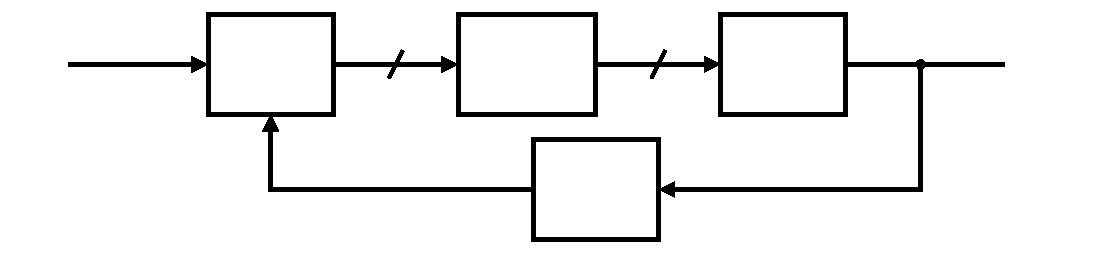
\includegraphics[scale=0.70000]{./figs/basic_adpll.pdf}\\
   % translate x=368 y=488 scale 0.38
   \putbox{1.09200in}{0.82600in}{1.20}{TDC}%
   \putbox{2.63200in}{0.24500in}{1.20}{$\div$ N}%
   \putbox{0.35700in}{0.97300in}{1.20}{$\Phi_{ref}$[n]}%
   \putbox{4.09500in}{0.97300in}{1.20}{$\Phi_{out}$[n]}%
   \putbox{2.19800in}{0.82600in}{1.20}{H$_{LF}$(z)}%
   \putbox{3.47900in}{0.82600in}{1.20}{DCO}%
   \putbox{1.67300in}{0.39200in}{1.20}{$\Phi_{div}$[n]}%
   \putbox{1.64500in}{1.02900in}{1.20}{e$_{\Phi}$[n]}%
   \putbox{2.92600in}{1.02900in}{1.20}{u[n]}%
   } % close 'parbox'
   } % close 'scalebox'
   \vspace{-\baselineskip} % this is not necessary, but looks better
\fontfamily{\rmdefault}\selectfont

	\caption{Basic ADPLL.}
	\label{fig:basic_adpll}
\end{figure}
\FloatBarrier
The basic architecture of an ADPLL is shown in figure \ref{fig:basic_adpll}. Here, compared to the continuous PLL, the phase detector has been replaced with a time to digital converter (TDC), the loop filter $\mathrm{H}_{LF}(s)$ with a discrete loop filter $\mathrm{H}_{LF}(z)$, and the VCO with a digitally controlled oscillator (DCO). In this architecture, the TDC, loop filter, and DCO are digital. 

\subsubsection{Divider}
A digital divider behaves nearly identical to the continuous case:
\begin{equation}
	\Phi_{div}[n] = \frac{\Phi_{out}[n]}{\mathrm{N}}
\end{equation}
Application of the z-transform:
\begin{equation}
	\frac{\Phi_{div}(z)}{\Phi_{out}(z)} = \frac{1}{\mathrm{N}}
\end{equation}
\subsubsection{TDC}
The TDC is a digital, quantized representation of the the phase detector. It takes input phase signals $\Phi_{div}$[n] and $\Phi_{ref}$[n], and outputs a digital phase error measurement word $e_\Phi[n]$. Figure \ref{fig:tdc} shows the basic TDC model architecture. A TDC will have limited resolution in phase, equivalent to M steps per reference cycle. This is a minimum step size in time of $\Delta t_{step}$ = $1/Mf_{ref}$. Since the output of the TDC is digital, the model applies a scale factor M$/2\pi$ and floor rounding, so 1 LSB of $e_\Phi[n]$ equates to $\Delta t_{step}$ timing error  between $\Phi_{div}$[n] and $\Phi_{ref}$[n].
\begin{figure}[htb!]
	\center\fontfamily{\sfdefault}\selectfont
% XCircuit output "tdc.tex" for LaTeX input from tdc.ps
\def\putbox#1#2#3#4{\makebox[0.00000in][l]{\makebox[#1][l]{}\raisebox{\baselineskip}[0.00000in][0.00000in]{\raisebox{#2}[0.00000in][0.00000in]{\scalebox{#3}{#4}}}}}
\def\rightbox#1{\makebox[0.00000in][r]{#1}}
\def\centbox#1{\makebox[0.00000in]{#1}}
\def\topbox#1{\raisebox{-0.60\baselineskip}[0.00000in][0.00000in]{#1}}
\def\midbox#1{\raisebox{-0.20\baselineskip}[0.00000in][0.00000in]{#1}}
   \scalebox{1}{
   \normalsize
   \parbox{3.50000in}{
   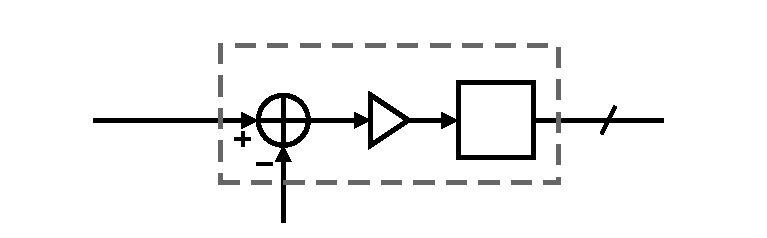
\includegraphics[scale=0.70000]{./figs/tdc.pdf}\\
   % translate x=432 y=396 scale 0.38
   \putbox{0.46200in}{0.63700in}{1.20}{$\Phi_{ref}$[n]}%
   \putbox{1.35100in}{0.08400in}{1.20}{$\Phi_{div}$[n]}%
   \putbox{2.68100in}{0.66500in}{1.20}{e$_\Phi$[n]}%
   \putbox{1.77800in}{0.70700in}{1.20}{\rotatebox{-360}{$\frac{\mathrm{M}}{2\pi}$}}%
   \putbox{1.47000in}{0.63700in}{1.20}{$\Phi_e$}%
   \putbox{2.18400in}{0.50400in}{1.20}{$\lfloor x\rfloor$}%
   \putbox{1.02900in}{0.95900in}{1.20}{TDC}%
   } % close 'parbox'
   } % close 'scalebox'
   \vspace{-\baselineskip} % this is not necessary, but looks better
\fontfamily{\rmdefault}\selectfont

	\caption{TDC model.}
	\label{fig:tdc}
\end{figure}
\begin{equation}
	e_\Phi[n] = \left\lfloor\frac{\mathrm{M}}{2\pi}(\Phi_{ref}[n] - \Phi_{div}[n])\right\rfloor
\end{equation}
For purposes of PLL transfer function calculation, the z-domain representation is as follows. Effects of quantization will be handled in section \ref{pn_theory}.
\begin{equation}
	e_\Phi(z) = \frac{\mathrm{M}}{2\pi}(\Phi_{ref}(z) - \Phi_{div}(z))
\end{equation}	
\FloatBarrier
\subsubsection{Loop Filter}
The loop filter design will be derived from the continuous PI-controller loop filter with optional peaking compensation (equation \ref{eq:pi_compensated_tf}) via application of the bilinear transform. The bilinear transform specifically allows for the conversion of a continuous transfer function to discrete representation, and vice versa. This, however is conditioned on satisfaction of Nyquist sampling criteria, and in the case of PLLs it is recommended that $f_s > 10\cdot\mathrm{BW}_{loop}$ to ensure transformation accuracy \cite{gardner_1980}. A high level of oversampling allows for the following definition of the bilinear transform, where 1/T=$f_{ref}$:
\begin{align*}
	z^{-1} &= e^{-sT} && \text{(definition of z-space)} \\
	&= \sum_{k=0}^\infty\frac{(-sT)^k}{k!} && \text{(exponential Taylor series)} \\
	&\approx 1-sT &&\text{(if $|sT| = 2\pi\mathrm{BW}_{loop}\cdot T << 1$)} \\
\end{align*}
Thus the bilinear transform identities are:
\begin{align}
	z^{-1} &= 1-sT\\
	s &= \frac{1}{T}(1-z^{-1}) \label{eq:s_to_z}
\end{align}
Applying \ref{eq:s_to_z} to equation \ref{eq:pi_compensated_tf} yields the z-domain loop filter:
\begin{align}
	\textnormal{H}_{LF}(z) = \left.\textnormal{H}_{LF}(s)\right\vert_{s=\frac{1}{T}(1-z^{-1})} = \left.\frac{K_i}{s}\frac{\left(\frac{s}{\omega_z} + 1\right)}{\left(\frac{s}{\omega_p} + 1\right)}\right\vert_{s=\frac{1}{T}(1-z^{-1})}\\
	= \frac{\omega_p}{\omega_z}\frac{k_iT}{(1-z^{-1})}\frac{(1+\omega_zT)-z^{-1}}{(1+\omega_pT) - z^{-1}(2+\omega_pT) + z^{-2}}\label{eq:z_lf}
\end{align}
Equation \ref{eq:z_lf} is converted to a digitally implementable representation via converting into the canonical representation of \ref{eq:canonical_z}, which determines the tap coefficients for the sampled-time difference equation \ref{eq:cananical_diff}. 
\begin{align}
	\textnormal{H}_{LF}(z) &= \frac{\sum_{j=0}^M b_jz^{-j}}{1+\sum_{k=1}^N a_kz^{-k}}\label{eq:canonical_z} \\
	y[n]&= -\sum_{k=1}^N a_ky[n-k] + \sum_{j=0}^M b_jx[n-j] \label{eq:cananical_diff}
\end{align}
Equation \ref{eq:cananical_diff} is directly implementable in digital hardware with a direct type 1 IIR filter shown in figure \ref{fig:filt_imple}, with the filter coefficients given by equations \ref{eq:a1}-\ref{eq:b1}. The filter coefficients must be quantized into finite resolution fixed point words for a complete digital implementation. Effects of quantization will be discussed in section \ref{pn_theory}.
\begin{figure}[htb!]
	\center\fontfamily{\sfdefault}\selectfont
% XCircuit output "filter_arch_tex.tex" for LaTeX input from filter_arch_tex.ps
\def\putbox#1#2#3#4{\makebox[0.00000in][l]{\makebox[#1][l]{}\raisebox{\baselineskip}[0.00000in][0.00000in]{\raisebox{#2}[0.00000in][0.00000in]{\scalebox{#3}{#4}}}}}
\def\rightbox#1{\makebox[0.00000in][r]{#1}}
\def\centbox#1{\makebox[0.00000in]{#1}}
\def\topbox#1{\raisebox{-0.60\baselineskip}[0.00000in][0.00000in]{#1}}
\def\midbox#1{\raisebox{-0.20\baselineskip}[0.00000in][0.00000in]{#1}}
   \scalebox{1}{
   \normalsize
   \parbox{5.54167in}{
   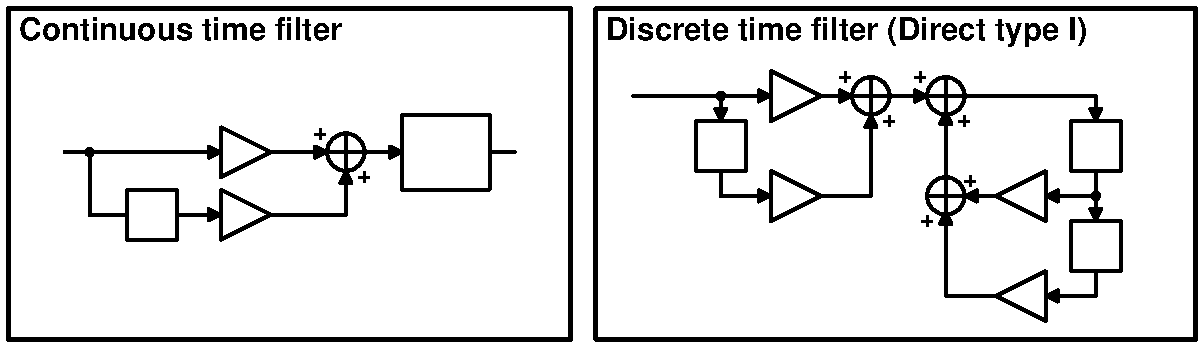
\includegraphics[scale=0.70000]{./figs/filter_arch_tex.pdf}\\
   % translate x=1728 y=944 scale 0.38
   \putbox{1.91800in}{0.90300in}{0.96}{$\frac{1}{\frac{s}{\omega_p} + 1}$}%
   \putbox{1.14800in}{1.01500in}{0.96}{$K_p$}%
   \putbox{1.14800in}{0.72800in}{0.96}{$K_i$}%
   \putbox{0.60900in}{0.58100in}{0.96}{$1/s$}%
   \putbox{0.25900in}{0.98700in}{0.96}{x[n]}%
   \putbox{2.35900in}{0.98700in}{0.96}{y[n]}%
   \putbox{2.92600in}{1.25300in}{0.96}{x[n]}%
   \putbox{5.17300in}{1.16200in}{0.96}{y[n]}%
   \putbox{3.26200in}{0.90300in}{0.96}{$z^{-1}$}%
   \putbox{3.73100in}{1.28100in}{0.96}{b$_0$}%
   \putbox{3.73100in}{0.81200in}{0.96}{b$_1$}%
   \putbox{5.01200in}{0.90300in}{0.96}{$z^{-1}$}%
   \putbox{5.01200in}{0.43400in}{0.96}{$z^{-1}$}%
   \putbox{4.60600in}{0.82600in}{0.96}{-a$_1$}%
   \putbox{4.59200in}{0.35700in}{0.96}{-a$_2$}%
   \putbox{5.17300in}{0.69300in}{0.96}{y[n-1]}%
   \putbox{5.15900in}{0.23100in}{0.96}{y[n-2]}%
   } % close 'parbox'
   } % close 'scalebox'
   \vspace{-\baselineskip} % this is not necessary, but looks better
\fontfamily{\rmdefault}\selectfont

	\caption{Implementation of filter.}
	\label{fig:filt_imple}
\end{figure}
			% y[n] = x[n]\frac{K_i\omega_pT}{\omega_z}\frac{1+\omega_zT}{1+\omega_pT} - x[n-1]\frac{K_i\omega_pT}{\omega_z}\frac{1}{1+\omega_pT} + y[n-1]\frac{2+\omega_pT}{1+\omega_pT} - y[n-2]\frac{1}{1+\omega_pT}\\
			% = a_0x[n] + a_1x[n-1] - b_1y[n-1] - b_2x[n-2] 
\begin{align}
	a_1 &= -\frac{2+\omega_pT}{1+\omega_pT}\label{eq:a1}\\
	a_2 &= \frac{1}{1+\omega_pT} \\
	b_0 &= \frac{K_i\omega_pT}{\omega_z}\frac{1+\omega_zT}{1+\omega_pT}\\
	b_1 &= \frac{K_i\omega_pT}{\omega_z}\frac{1}{1+\omega_pT}\label{eq:b1}
\end{align}
\subsubsection{DCO}
The DCO is modeled in discrete time as a recursive phase integrator, dependent on the DCO gain $K_{DCO}$, which provides the frequency tuning per LSB of the oscillator, the input oscillator tuning word u[n], and the sampling period T.
\begin{equation}
	\Phi_{out}[n] = \Phi_{out}[n-1] + 2\pi K_{DCO}u[n]T
\end{equation}
Application of the z-transform yields:
\begin{equation}
	\frac{\Phi_{out}(z)}{u(z)} = \frac{2\pi K_{DCO}T}{1-z^{-1}}
\end{equation}
Application of the bilinear transform to the DCO transfer function yields:
\begin{equation}
	\frac{\Phi_{out}(s)}{u(s)} = \frac{2\pi K_{DCO}T}{1-(1-sT)} = \frac{2\pi K_{DCO}}{s} 
\end{equation}
\subsubsection{Discrete-time PLL transfer function}
\begin{figure}[htb!]
	\center\fontfamily{\sfdefault}\selectfont
% XCircuit output "discrete_pll.tex" for LaTeX input from discrete_pll.ps
\def\putbox#1#2#3#4{\makebox[0.00000in][l]{\makebox[#1][l]{}\raisebox{\baselineskip}[0.00000in][0.00000in]{\raisebox{#2}[0.00000in][0.00000in]{\scalebox{#3}{#4}}}}}
\def\rightbox#1{\makebox[0.00000in][r]{#1}}
\def\centbox#1{\makebox[0.00000in]{#1}}
\def\topbox#1{\raisebox{-0.60\baselineskip}[0.00000in][0.00000in]{#1}}
\def\midbox#1{\raisebox{-0.20\baselineskip}[0.00000in][0.00000in]{#1}}
   \scalebox{1}{
   \normalsize
   \parbox{6.88333in}{
   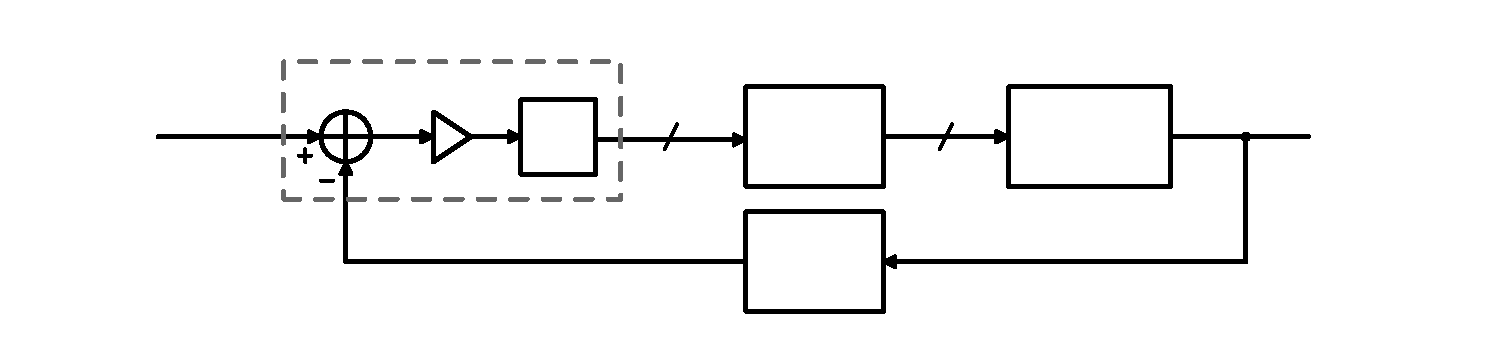
\includegraphics[scale=0.70000]{./figs/discrete_pll.pdf}\\
   % translate x=512 y=508 scale 0.38
   \putbox{0.74200in}{1.04300in}{1.20}{$\Phi_{ref}$[n]}%
   \putbox{2.17000in}{0.47600in}{1.20}{$\Phi_{div}$[n]}%
   \putbox{3.00300in}{1.07800in}{1.20}{e$_\Phi$[n]}%
   \putbox{2.06500in}{1.12000in}{1.20}{\rotatebox{-360}{$\frac{\mathrm{M}}{2\pi}$}}%
   \putbox{1.75700in}{1.04300in}{1.20}{$\Phi_e$}%
   \putbox{2.47800in}{0.91700in}{1.20}{$\lfloor x\rfloor$}%
   \putbox{1.32300in}{1.36500in}{0.90}{TDC}%
   \putbox{3.55600in}{0.91700in}{1.20}{H$_{LF}$(z)}%
   \putbox{4.28400in}{1.07800in}{1.20}{u[n]}%
   \putbox{4.73200in}{0.93100in}{1.20}{$\frac{2\pi K_{DCO}T}{1-z^{-1}}$}%
   \putbox{5.55100in}{1.04300in}{1.20}{$\Phi_{out}$[n]}%
   \putbox{3.62600in}{0.32900in}{1.20}{$\div$ N}%
   \putbox{4.70400in}{1.23200in}{0.90}{DCO}%
   } % close 'parbox'
   } % close 'scalebox'
   \vspace{-\baselineskip} % this is not necessary, but looks better
\fontfamily{\rmdefault}\selectfont

	\caption{Discrete time PLL model.}
	\label{fig:discrete_pll2}
\end{figure}
\FloatBarrier
The transfer function for the discrete-time PLL can be computed in the z-domain, and also approximated continuously. The open loop z-domain transfer function is:
\begin{align}
\mathrm{OL}(z) = \mathrm{H}_{TDC}(z)\mathrm{H}_{LF}(z)\mathrm{H}_{DCO}(z)\mathrm{H}_{DIV}(z) = \\
2\pi K_{DCO}K_iT^2\frac{\mathrm{M}}{\mathrm{N}}\frac{\omega_p}{\omega_z}\frac{(1+\omega_zT)-z^{-1}}{(1+\omega_pT) - z^{-1}(3+2\omega_pT) + z^{-2}(3+\omega_pT) - z^{-3}}\label{eq:z_lf}
\end{align}
The closed loop z-domain PLL phase transfer function is:
\begin{align}
\frac{\Phi_{out}(z)}{\Phi_{ref}(z)} = \frac{\mathrm{H}_{DIV}(z)^{-1}\mathrm{OL}(z)}{1+\mathrm{OL}(z)} = \\
\frac{2\pi K_{DCO}K_iT^2\mathrm{M}\frac{\omega_p}{\omega_z}(1+\omega_zT)-z^{-1}}{(1+\omega_pT + 2\pi K_{DCO}K_iT^2\frac{\mathrm{M}}{\mathrm{N}}\frac{\omega_p}{\omega_z}(1+\omega_zT))- z^{-1}(3+2\omega_pT+2\pi K_{DCO}K_iT^2\frac{\mathrm{M}}{\mathrm{N}}\frac{\omega_p}{\omega_z})+ z^{-2}(3+\omega_pT) - z^{-3}}
\end{align}
The s-domain approximation of the transfer function is:
\begin{align}
\mathrm{OL}(s) = \mathrm{H}_{TDC}(s)\mathrm{H}_{LF}(s)\mathrm{H}_{DCO}(s)\mathrm{H}_{DIV}(s) = \frac{\mathrm{M}}{\mathrm{N}}\frac{K_{DCO}K_i}{s^2} \frac{\left(\frac{s}{\omega_z} + 1\right)}{\left(\frac{s}{\omega_p} + 1\right)}
\end{align}
And in closed loop configuration the PLL phase transfer function is:
\begin{align}
\frac{\Phi_{out}(z)}{\Phi_{ref}(z)} = \frac{\mathrm{H}_{DIV}(z)^{-1}\mathrm{OL}(z)}{1+\mathrm{OL}(z)} = \frac{\mathrm{M}K_{DCO}K_i\left(\frac{s}{\omega_z} + 1\right)}{s^3\frac{1}{\omega_z} + s^2 + \frac{\mathrm{M}}{\mathrm{N}}K_{DCO}K_i\left(\frac{s}{\omega_z} + 1\right)}
\end{align}
Incidentally, the s-domain approximation is significantly simpler and will is preferred in this paper for purposes of analysis.


\subsection{PLL Noise} \label{pn_theory}
The predominant sources of noise in the discrete-time ADPLL are chiefly quantization (in the TDC, loop filter, and DCO), along with thermal noise (in the DCO, divider and TDC). The noise generated by these quantization sources will be discussed in the following sections.

\subsubsection{TDC noise}
The predominant phase noise source in the TDC is due to quantization. A straightforward approach to model quantization noise is to utilize the model of figure \ref{fig:tdc_add_pn} to represent quantization.
\hspace{-20em}\begin{figure}[htb!]
    \centering
    \begin{subfigure}{0.5\textwidth}
        \centering
        \fontfamily{\sfdefault}\selectfont
% XCircuit output "tdc.tex" for LaTeX input from tdc.ps
\def\putbox#1#2#3#4{\makebox[0.00000in][l]{\makebox[#1][l]{}\raisebox{\baselineskip}[0.00000in][0.00000in]{\raisebox{#2}[0.00000in][0.00000in]{\scalebox{#3}{#4}}}}}
\def\rightbox#1{\makebox[0.00000in][r]{#1}}
\def\centbox#1{\makebox[0.00000in]{#1}}
\def\topbox#1{\raisebox{-0.60\baselineskip}[0.00000in][0.00000in]{#1}}
\def\midbox#1{\raisebox{-0.20\baselineskip}[0.00000in][0.00000in]{#1}}
   \scalebox{1}{
   \normalsize
   \parbox{3.50000in}{
   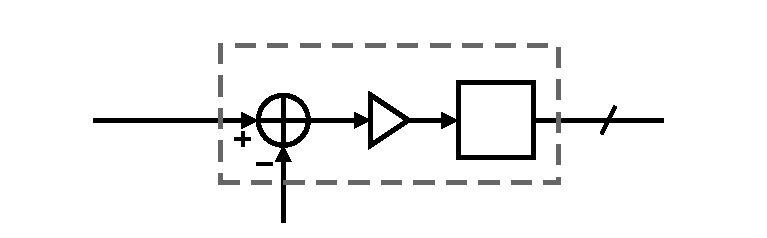
\includegraphics[scale=0.70000]{./figs/tdc.pdf}\\
   % translate x=432 y=396 scale 0.38
   \putbox{0.46200in}{0.63700in}{1.20}{$\Phi_{ref}$[n]}%
   \putbox{1.35100in}{0.08400in}{1.20}{$\Phi_{div}$[n]}%
   \putbox{2.68100in}{0.66500in}{1.20}{e$_\Phi$[n]}%
   \putbox{1.77800in}{0.70700in}{1.20}{\rotatebox{-360}{$\frac{\mathrm{M}}{2\pi}$}}%
   \putbox{1.47000in}{0.63700in}{1.20}{$\Phi_e$}%
   \putbox{2.18400in}{0.50400in}{1.20}{$\lfloor x\rfloor$}%
   \putbox{1.02900in}{0.95900in}{1.20}{TDC}%
   } % close 'parbox'
   } % close 'scalebox'
   \vspace{-\baselineskip} % this is not necessary, but looks better
\fontfamily{\rmdefault}\selectfont

        \caption{TDC Model.}
        \label{fig:tdc1}
    \end{subfigure}%
    \begin{subfigure}{0.5\textwidth}
        \centering
        \fontfamily{\sfdefault}\selectfont
% XCircuit output "tdc_quant.tex" for LaTeX input from tdc_quant.ps
\def\putbox#1#2#3#4{\makebox[0.00000in][l]{\makebox[#1][l]{}\raisebox{\baselineskip}[0.00000in][0.00000in]{\raisebox{#2}[0.00000in][0.00000in]{\scalebox{#3}{#4}}}}}
\def\rightbox#1{\makebox[0.00000in][r]{#1}}
\def\centbox#1{\makebox[0.00000in]{#1}}
\def\topbox#1{\raisebox{-0.60\baselineskip}[0.00000in][0.00000in]{#1}}
\def\midbox#1{\raisebox{-0.20\baselineskip}[0.00000in][0.00000in]{#1}}
   \scalebox{1}{
   \normalsize
   \parbox{3.50000in}{
   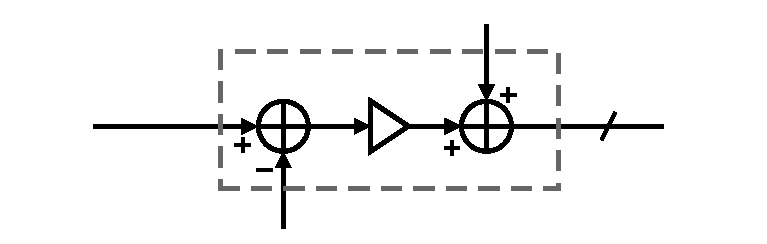
\includegraphics[scale=0.70000]{./figs/tdc_quant.pdf}\\
   % translate x=432 y=396 scale 0.38
   \putbox{0.46200in}{0.63700in}{1.20}{$\Phi_{ref}$[n]}%
   \putbox{1.35100in}{0.08400in}{1.20}{$\Phi_{div}$[n]}%
   \putbox{2.68100in}{0.66500in}{1.20}{e$_\Phi$[n]}%
   \putbox{1.77800in}{0.70700in}{1.20}{\rotatebox{-360}{$\frac{\mathrm{M}}{2\pi}$}}%
   \putbox{1.47000in}{0.63700in}{1.20}{$\Phi_e$}%
   \putbox{2.31700in}{0.97300in}{1.20}{q$_{TDC}$[n]}%
   \putbox{1.02900in}{0.95900in}{1.20}{TDC}%
   } % close 'parbox'
   } % close 'scalebox'
   \vspace{-\baselineskip} % this is not necessary, but looks better
\fontfamily{\rmdefault}\selectfont

        \caption{TDC additive noise model.}
        \label{fig:tdc_add_pn}
    \end{subfigure}
    % \caption{Approximate model for ring oscillator inverter delay cell.}
    \label{fig:tdc_pn_model}
\end{figure}
\FloatBarrier
Using this model, the quantized signal $e_\Phi$[n] is the sum of the its unquantized representation $\Phi_e\frac{\mathrm{M}}{2\pi}$ with a quantization error signal $\mathrm{q}_{TDC}[n]$. Figure \ref{fig:quantization} illustrates this process.
\begin{figure}[htb!]
	\center\fontfamily{\sfdefault}\selectfont
% XCircuit output "quantization.tex" for LaTeX input from quantization.ps
\def\putbox#1#2#3#4{\makebox[0.00000in][l]{\makebox[#1][l]{}\raisebox{\baselineskip}[0.00000in][0.00000in]{\raisebox{#2}[0.00000in][0.00000in]{\scalebox{#3}{#4}}}}}
\def\rightbox#1{\makebox[0.00000in][r]{#1}}
\def\centbox#1{\makebox[0.00000in]{#1}}
\def\topbox#1{\raisebox{-0.60\baselineskip}[0.00000in][0.00000in]{#1}}
\def\midbox#1{\raisebox{-0.20\baselineskip}[0.00000in][0.00000in]{#1}}
   \scalebox{1}{
   \normalsize
   \parbox{4.24010in}{
   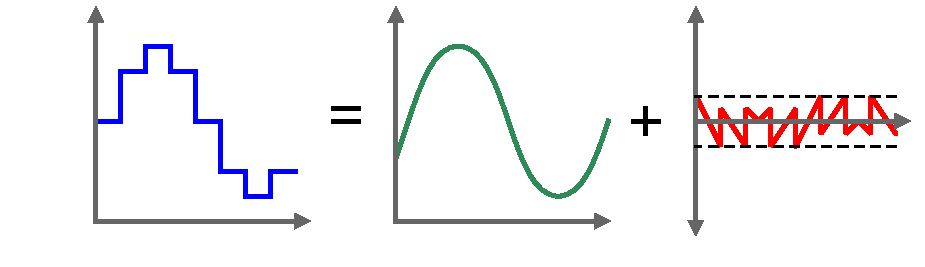
\includegraphics[scale=0.70000]{./figs/quantization.pdf}\\
   % translate x=304 y=240 scale 0.38
   \putbox{0.04200in}{1.09200in}{0.96}{$e_\Phi$[n]}%
   \putbox{1.32300in}{0.04200in}{0.96}{t=nT}%
   \putbox{1.32300in}{1.09200in}{0.96}{$\frac{\mathrm{M}}{2\pi}\Phi_e$[n]}%
   \putbox{2.77900in}{0.04200in}{0.96}{\rotatebox{-360}{t}}%
   \putbox{4.24200in}{0.50400in}{0.96}{t}%
   \putbox{2.72300in}{1.09200in}{0.96}{q$_{\mathrm{TDC}}$[n]}%
   \putbox{3.47900in}{0.85400in}{0.96}{$+\Delta/2$}%
   \putbox{3.47900in}{0.44800in}{0.96}{$-\Delta/2$}%
   } % close 'parbox'
   } % close 'scalebox'
   \vspace{-\baselineskip} % this is not necessary, but looks better
\fontfamily{\rmdefault}\selectfont

	\caption{Quantization as via additive error signal.}
	\label{fig:quantization}
\end{figure}
\FloatBarrier
The quantization noise signal has the statistical property that it is uniformly distributed in the range $[-\Delta/2, \Delta/2]$, i.e. $P_q(Q=q) =\mathrm{U}(-\Delta/2, \Delta/2)$ if $\Delta$ is the quantization step size. The power of the TDC quantization noise signal is:
\begin{equation}\label{eq:tdc_noise}
\sigma_{q_{TDC}}^2 = \int_{-\infty}^\infty q^2P_q(Q=q)dq =  \int_{-\Delta/2}^{\Delta/2}\frac{q^2}{\Delta}dq = \frac{\Delta^2}{12}
\end{equation}
Since $e_\Phi$[n] is digital signal, the minimum step size is $\Delta$=1 LSB. The TDC quantization noise power is therefore $\sigma_{q_{TDC}}^2 = 1/12$ LSB$^2$. The po
If the quantization noise is assumed to be white, and the TDC is sampled at $f_{ref}$, the quantization PSD is:
\begin{equation}
S_{q_{TDC}} = \frac{P_{q_{TDC}}}{\Delta f} = \frac{\sigma_{q_{TDC}}^2}{f_{ref}} = \frac{\Delta^2}{12f_{ref}} = \frac{1}{12f_{ref}} \hspace{1em}\frac{[\text{LSB}]^2}{[\text{Hz}]}
\end{equation}

\subsubsection{DCO noise}
\begin{figure}[htb!]
	\center\fontfamily{\sfdefault}\selectfont
% XCircuit output "dco_noise.tex" for LaTeX input from dco_noise.ps
\def\putbox#1#2#3#4{\makebox[0.00000in][l]{\makebox[#1][l]{}\raisebox{\baselineskip}[0.00000in][0.00000in]{\raisebox{#2}[0.00000in][0.00000in]{\scalebox{#3}{#4}}}}}
\def\rightbox#1{\makebox[0.00000in][r]{#1}}
\def\centbox#1{\makebox[0.00000in]{#1}}
\def\topbox#1{\raisebox{-0.60\baselineskip}[0.00000in][0.00000in]{#1}}
\def\midbox#1{\raisebox{-0.20\baselineskip}[0.00000in][0.00000in]{#1}}
   \scalebox{1}{
   \normalsize
   \parbox{3.56562in}{
   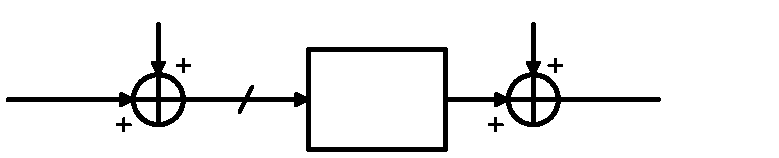
\includegraphics[scale=0.70000]{./figs/dco_noise.pdf}\\
   % translate x=-384 y=320 scale 0.38
   \putbox{1.02900in}{0.39200in}{0.96}{u[n]}%
   \putbox{1.48400in}{0.24500in}{0.96}{$\frac{2\pi K_{DCO}T}{1-z^{-1}}$}%
   \putbox{2.66700in}{0.34300in}{0.96}{$\Phi_{out}$[n]}%
   \putbox{0.78400in}{0.60900in}{0.96}{q$_{OTW}$[n]}%
   \putbox{0.18200in}{0.37800in}{0.96}{$\hat{\textnormal{u}}$[n]}%
   \putbox{2.54800in}{0.62300in}{0.96}{$\Phi_{n_{DCO}}$[n]}%
   } % close 'parbox'
   } % close 'scalebox'
   \vspace{-\baselineskip} % this is not necessary, but looks better
\fontfamily{\rmdefault}\selectfont

	\caption{DCO additive noise model.}
	\label{fig:quantization}
\end{figure}
\FloatBarrier
Noise in the DCO is from quantization of the oscillator tuning word (OTW), and from thermal and stochastic sources. In the digital PLL, the OTW is quantized in loop filter, so this source of noise will be analyzed in the loop filter section. Thus oscillator thermal noise will be considered.
\begin{figure}[htb!]
	\center\fontfamily{\sfdefault}\selectfont
% XCircuit output "aperture_noise.tex" for LaTeX input from aperture_noise.ps
\def\putbox#1#2#3#4{\makebox[0.00000in][l]{\makebox[#1][l]{}\raisebox{\baselineskip}[0.00000in][0.00000in]{\raisebox{#2}[0.00000in][0.00000in]{\scalebox{#3}{#4}}}}}
\def\rightbox#1{\makebox[0.00000in][r]{#1}}
\def\centbox#1{\makebox[0.00000in]{#1}}
\def\topbox#1{\raisebox{-0.60\baselineskip}[0.00000in][0.00000in]{#1}}
\def\midbox#1{\raisebox{-0.20\baselineskip}[0.00000in][0.00000in]{#1}}
   \scalebox{1}{
   \normalsize
   \parbox{2.24062in}{
   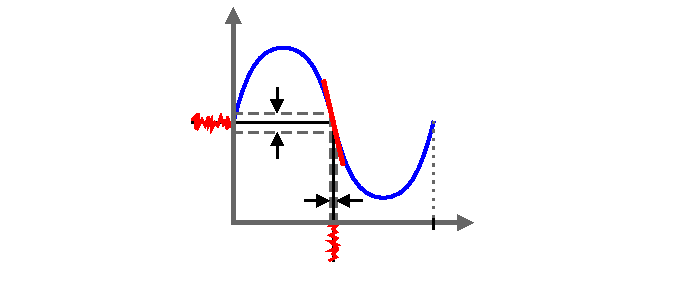
\includegraphics[scale=0.90000]{./figs/aperture_noise.pdf}\\
   % translate x=-108 y=240 scale 0.38
   \putbox{1.87200in}{0.16200in}{0.96}{\rotatebox{-360}{$\Phi$}}%
   \putbox{0.07200in}{1.40400in}{0.96}{V$_{out}$}%
   \putbox{0.63000in}{1.13400in}{0.96}{$\sigma_{v_n}$}%
   \putbox{0.61200in}{0.40500in}{0.96}{$\sigma_{\Phi_n}$}%
   \putbox{0.05400in}{1.06200in}{0.60}{Thermal }%
   \putbox{0.12600in}{0.97200in}{0.60}{noise}%
   \putbox{0.71100in}{0.14400in}{0.60}{Phase }%
   \putbox{0.72900in}{0.05400in}{0.60}{noise}%
   \putbox{1.58400in}{0.14400in}{0.60}{\rotatebox{-360}{$2\pi$}}%
   \putbox{0.40500in}{0.14400in}{0.60}{$0$}%
   } % close 'parbox'
   } % close 'scalebox'
   \vspace{-\baselineskip} % this is not necessary, but looks better
\fontfamily{\rmdefault}\selectfont

	\caption{Thermal to phase noise conversion.}
	\label{fig:quantization}
\end{figure}
\FloatBarrier
 Noise from circuit and supply noise can be realized as an additive voltage component to the oscillator waveform $V_{osc}(t)$, with variance $\sigma_{V_n}^2$. As $V_{osc}(t)$ will have a finite derivative, a small additive noise signal $v_{n}(t)$ will be coupled into the time domain as a phase noise disturbance $\delta\Phi_{n}$ in the oscillator phase. At any point in time, assuming Gaussian white noise, $\delta\Phi_{n}$ is sampled from the following distribution:
 \begin{equation}
 \delta\Phi_{n} \sim \left.\text{Norm}\left(\mu=0, \sigma=\left(\frac{dV(\Phi)}{d\Phi}\right)^{-1}\sigma_{v_n}\right)\right\vert_{\Phi=\omega_{osc}t}
 \end{equation} 
The phase disturbance $\delta\Phi_{n}(t)$ at t is independent of all other points in time. If the phase of the oscillator is analyzed with discrete step $T$:
\begin{equation}
\Phi_{out}[n] = \Phi_{out}[n-1] + \omega_{osc}T + \delta\Phi_n[\Phi=n\omega_{osc} T]
\end{equation}
The contribution only due to phase disturbance, i.e. phase noise $\Phi_n$[n]:
\begin{equation}
\Phi_{n}[n] = \Phi_{out}[n] - \omega_{osc}T = \Phi_{out}[n-1] + \delta\Phi_n[n|\Phi=n\omega_{osc}T]
\end{equation}
Notice this takes the form of a random walk signal. Computing the z-transform
\begin{equation}
\Phi_{n}(z) = \frac{\delta\Phi_n(z)}{1-z^{-1}}
\end{equation}
Application of the bilinear transform can be used to approximate the continuous noise spectrum:
\begin{equation}
\left.\Phi_{n}(z)\right\vert_{z=1-sT} = \left.\frac{\delta\Phi_n(z)}{1-z^{-1}}\right\vert_{z=1-sT} = \frac{\delta\Phi_n(z=1-sT)}{sT}
\end{equation}
The phase noise PSD is therefore:
\begin{equation}
S_{\Phi n_{DCO}}(\omega)= \left|\frac{\delta\Phi_n(z=1-j\omega T)}{j\omega T}\right|^2 = \frac{1}{\omega^2}\left|\frac{\delta\Phi_n(z=1-j\omega T)}{T}\right|^2
\end{equation}
Following that the phase disturbance signal $\delta\Phi_{n}(t)$ is white spectrum, a value for its power $S_{0\Phi n_{DCO}}$ can be defined as such:
\begin{equation}
S_{0\Phi n_{DCO}} = \lim_{T\to0} \mathrm{Var}\left( \left|\frac{\delta\Phi_n(z=1-j\omega T)}{T}\right|^2 \right)
\end{equation}
The value for $S_{0\Phi n_{DCO}}$ is highly dependent on implementation and is best extracted via simulation or physical measurement by fitting the following:
\begin{equation}
S_{\Phi n_{DCO}}(\omega)= \frac{S_{0\Phi n_{DCO}}}{\omega^2}
\end{equation}
\subsubsection{Divider noise}
Divider noise is manifested as jitter on the the output signal, due to thermal noise coupling from voltage to phase. If the divider is a digital circuit, with edge rate $dV/dt$, and subject to thermal noise in the form of a  voltage $v_n$, with noise power of $\sigma_{v_n}^2$, the phase noise (jitter) conferred is:
\begin{equation}
\sigma_{\Phi n_{DIV}} = \omega_{ref}\sigma_{t n_{DIV}}  =\omega_{ref}\left(\frac{dV}{dt}\right)^{-1}\sigma_{v_n}
\end{equation}
Thus the power is:
\begin{equation}
S_{\Phi n_{DIV}} = \omega^2_{ref}\sigma^2_{t n_{DIV}}  =\omega^2_{ref}\left(\frac{dV}{dt}\right)^{-2}\sigma_{v_n}^2
\end{equation}

\subsubsection{Loop filter noise}
Loop filter noise is principally from quantization in the digital case. In the digital loop filter, the mathematical operations are carried out with finite precision, and thus rounding errors occur. Here, an architecture with B bits in each fixed point word throughout the loop filter is assumed for analysis. 

\subsubsection{PLL output-referred noise}\label{pn_noise_psd}
In terms of analysis, PLL noise referred to the PLL output is of most interest. In this case, the noise is defined in terms of phase noise $\Phi_{n}$, or an unwanted added component to the oscillator phase signal $\Phi_{osc}=\omega_{osc}t$. The PLL output phase signal $\Phi_{out}$ is therefore:
\begin{equation}
	\Phi_{out}(t) = \Phi_{osc}(t) + \Phi_{n}(t) = \omega_{osc}t + \Phi_{n}(t) 
\end{equation}
In analyzing phase noise, the noise power spectral density of the PLL output is of most interest. To compute this, an output voltage waveform of the PLL must defined. Given an amplitude $A_0$:
\begin{equation}
V_{out} = \Re\left(A_0e^{j\Phi_{out}(t)}\right) = \Re\left(A_0e^{j\omega_{osc}t}e^{j\Phi_{n}(t)}\right)
\end{equation}
Assuming the phase noise signal is zero mean, $\mathbb{E}[\Phi_{n}(t)]=0$, and the power of phase noise signal is small, $\mathrm{Var}[\Phi_{n}(t)] << 1$, then the approximation $e^{j\Phi_{n}(t)} = 1 + j\Phi_{n}(t)$ can be applied.
\begin{align}
V_{out} = \Re\left(A_0e^{j\omega_{osc}t}e^{j\Phi_{n}(t)}\right) = \Re\left(A_0e^{j\omega_{osc}t} +j\Phi_{n}(t)A_0e^{j\omega_{osc}t}\right)\\
= A_0\cos(\omega_{osc}t) - \Phi_{n}(t)A_0\sin(\omega_{osc}t)
\end{align}
The result is a carrier cosine signal, and an orthogonal sine signal modulated by the phase noise $\Phi_{n}$. From this, the spectral density of the phase noise relative to the carrier can be estimated. Power spectral density is computed as such, assuming the carrier and the phase noise signal components are uncorrelated:
\begin{equation}
S_{V_{out}} = |\mathcal{F}\{V_{out}(t)\}|^2 = A_0^2|\mathcal{F}\{\cos(\omega_{osc}t)\}|^2 + A_0^2|\Phi_{n}(\omega)*\mathcal{F}\{\sin(\omega_{osc}t)\}|^2
\end{equation}
If single side band (SSB) noise power spectral density $\mathcal{L}(\Delta f)$ is defined as the phase noise PSD at offset $\Delta f$ from the carrier frequency $f_{osc}$, normalized to the carrier power:
\begin{equation}
\mathcal{L}(\Delta f) = |\Phi_{n}(2\pi\Delta f)|^2 = |\mathcal{F}\{\Phi_{n}(t)\}|^2= S_{\Phi_{n}}(\Delta f)
\end{equation}
Thus, the PLL output PSD noise relative to the carrier can be computed as the PSD of the phase noise signal $\Phi_{n}(t)$.

\subsubsection{PLL noise sensitivity transfer functions}
Having models for noise of generated by each PLL component, noise sensitivity transfer functions must be computer to refer each noise source to the PLL output in terms of phase. After which, the output noise PSD can be inferred based on the output phase signal, following the theory of section \ref{pn_noise_psd}. An important assumption is made, in that every noise source within the PLL is independent, so that their individual noise powers can be summed at the PLL output to compute the overall PLL output noise.

 and a method to calculate noise power spectral density from the output phase signal


All noise uncorrelated.

Plot of BW vs 
fasf
Generic theory of PLL
Discrete PLL
Noise theory
